\section{PID regulator koefficienter}
Ved brug af PID tool og simulink i matlab fundet frem til koefficienterne i \ref{PID_test14}.
Disse koefficienter er testet og plottet i Figur \ref{PID_test14_plot}.
Dette opfylder ikke de krav som der er sat i krav specifikationen.
Ziegler-Nichols metoden viste sig at være for aggressiv og resulterede i en binær regulator.

Reguleringssløjferne er testet ved at plotte loggen og se den maksimale fejl.
Systemet blev altid sat i samme start position ved funktionen som peger det første koordinat i testen.

\begin{figure}[h!]
\centering
\begin{tabu}{l|[1.25pt]c|c|c}
      & \(K_P\) & \(K_I\) & \(K_D\)\\\tabucline[1.25pt]{-}
Tilt  & 74,4933 & 435,0662 & 0,248960\\\hline
Pan   & 37,1740 &  33,3610 & 0,215658
\end{tabu}
\captionsetup{type=table}
\caption[Regulator koefficienter brugt i test]{Regulator koefficienter brugt til test af system.}
\label{PID_test14} 
\end{figure}

\begin{figure}
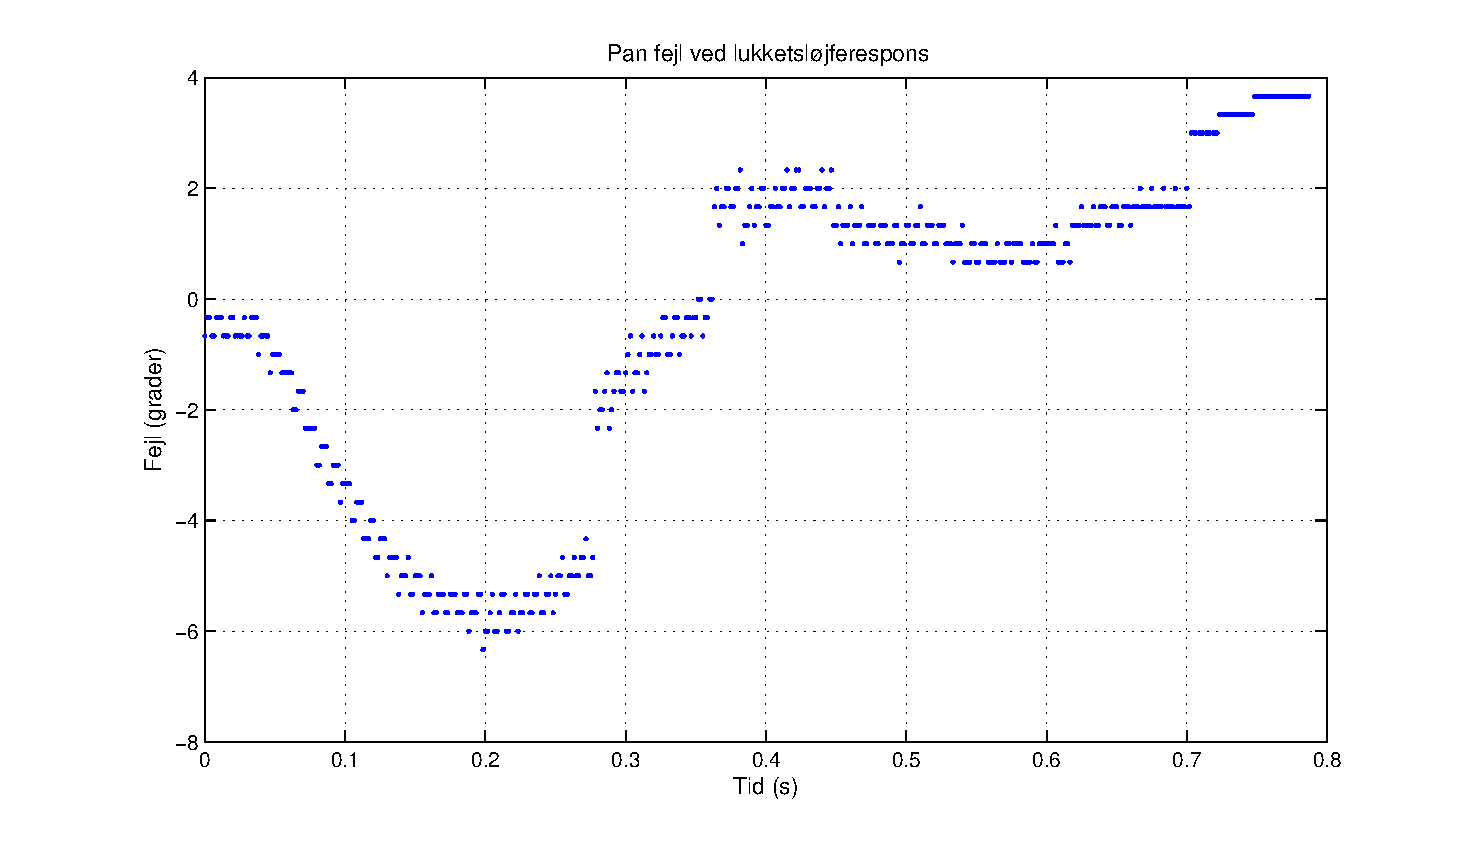
\includegraphics[width=1\textwidth]{./graphics/error_pan.eps}
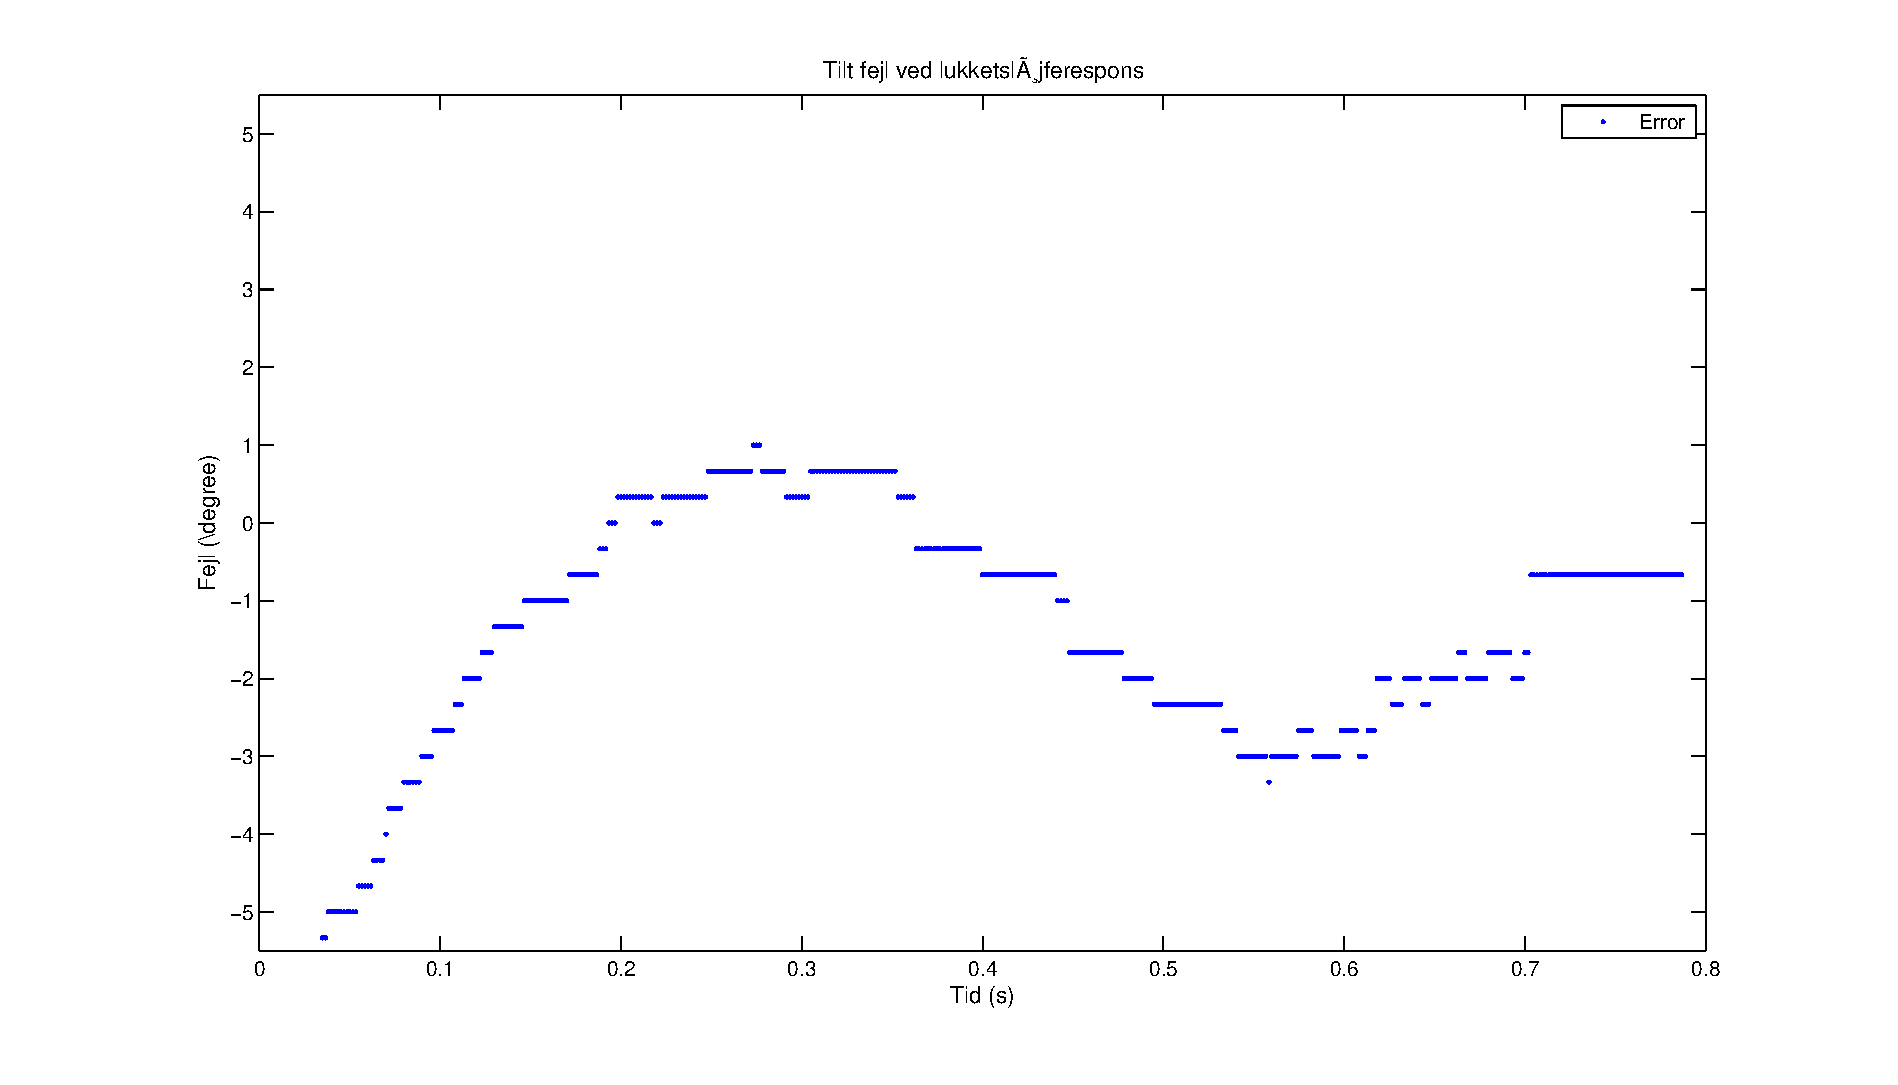
\includegraphics[width=1\textwidth]{./graphics/error_tilt.eps}
\caption[PID controller koefficienter]{Fejl målt i grader for PID controller med koefficienterne beskrevet i tabel \ref{PID_test14}.} \label{PID_test14_plot}
\end{figure}


\subsection{Optimering af controller/koefficienter}
